\section{Maintenance, regulation and compliance}

\begin{frame}{Rationale}
  \begin{itemize}
    \item "Cybersecurity" has been a rapidly growing concern
    \item The stakes are high:
    \begin{itemize}
      \item Reputation
      \item Downtime
      \item Money (blackmail, ransomware)
    \end{itemize}
    \item You can actually buy cybersecurity insurance
    % Think e.g. of the Equifax data breach, or Pole Emploi
    \item Some vulnerabilities have wide-reaching consequences for everyone
    \item Predictably, this has led to produce standards and legislation
  \end{itemize}
\end{frame}

\begin{frame}{Examples}
  \begin{itemize}
    \item standards
    \begin{itemize}
      \item ISO 27001
      \item NIST standards, such as
      \begin{itemize}
        \item the Federal Information Processing Standard (FIPS)
        \item the Advanced Encryption Standard (AES)
      \end{itemize}
      \item Common Criteria
    \end{itemize}
    \item laws
    \begin{itemize}
      \item Federal Information Security Modernization Act (FISMA)
      \item The Cyber Resilience Act (\href{https://eur-lex.europa.eu/legal-content/EN/TXT/?uri=CELEX\%3A02024R2847-20241120}{CRA})
    \end{itemize}
  \end{itemize}
\end{frame}

\subsection{Vulnerability frameworks}

\begin{frame}{Vulnerability taxonomy}
  \begin{itemize}
    \item A Vulnerability is a rather high-level concept
    \item Very different phenomena can be deemed a vulnerability:
    \begin{itemize}
      \item Having a deprecated feature still present in a UI
      \item Using HTTP
      \item Use-after-frees
      \item etc...
    \end{itemize}
    \item The MITRE corporation has a categorization of vulnerabilities by category:
          the \href{https://cwe.mitre.org/}{Common Weakness Enumeration (CWE)}
    \item CWE uses different categories to organize vulnerabilities
  \end{itemize}
\end{frame}

\begin{frame}{Vulnerability databases}
  \begin{itemize}
    \item Idea: central repository listing published vulnerabilities
    \item The main problem here is maintenance
    \item The reference was the U.S National Vulnerability Database (NVD)
    \begin{itemize}
      \item Funding issues have fragilized NVD as a reliable source
    \end{itemize}
    \item China has 2 databases: CNVD and CNNVD
    \begin{itemize}
      \item Both require accounts and can be difficult to navigate 
    \end{itemize}
    \item The EU has started the \href{https://euvd.enisa.europa.eu/search}{EUVD} in 2025
    \begin{itemize}
      \item Uses UUIDs for vendors and products
      \item Version ranges are not super trivial to parse
    \end{itemize}
  \end{itemize}
\end{frame}

\begin{frame}{The CVE program}
  \begin{itemize}
    \item CVE stands for "Common Vulnerabilities and Exposures"
    \item Has been operated by MITRE with US government funding
    \item This funding has had ups and downs in 2025, which has led to data quality issues
    \item \href{https://www.cve.org/programorganization/cnas}{CVE Numbering Authorities (CNAs)}
          can reserve and assign CVE numbers within their scope
    \item The Linux kernel team became a CNA in early 2024
    \item This is the program that serves as a base for the NVD
    \item Usually contains mostly rudimentary information at first
    \item Database is cached into a \href{https://github.com/CVEProject/cvelistV5}{github repo}
  \end{itemize}
\end{frame}

\begin{frame}{Common Vulnerability Scoring System (CVSS)}
  \begin{itemize}
    \item Open Framework published by FIRST
          (\href{https://www.first.org/cvss/specification-document}{specification})
    \item Current version is 4 since November 2023
    \item Usually, CVE records will use 1 or 2 versions of CVSS, depending on publication date
    \item CVSS results in:
    \begin{itemize}
      \item A "vector" representing the values of a discrete set of metrics
      \item A score between 0 and 10, which is a numerical conversion of the vector
    \end{itemize}
    \item The score is the result of a complex-ish
          \href{https://github.com/FIRSTdotorg/cvss-v4-calculator}{computation}
          (\href{https://redhatproductsecurity.github.io/cvss-v4-calculator/}{online calculator})
%    \code{CVSS:4.0/AV:N/AC:L/AT:N/PR:N/UI:N/VC:N/VI:N/VA:H/SC:N/SI:N/SA:N}
%    \code{CVSS:3.1/AV:N/AC:L/PR:N/UI:N/S:U/C:N/I:N/A:H}
  \end{itemize}
\end{frame}

\begin{frame}{Exploitation Predictability Scoring System (EPSS)}
  \begin{itemize}
    \item Relatively recent (2021) effort
    \item Backed by FIRST
    \item Gives an estimated probability of the vulnerability being exploited within the next 30 days
    \item Uses machine learning to correlate exploit activity to vulnerabilities
    \item Relies on closed-source data from industry partners re: exploitation
    \item One big question here is how big the blind spot due to the
          incompleteness of the exploitation data is
  \end{itemize}
\end{frame}

\begin{frame}[fragile]
  \frametitle{Common Platform Enumerations (CPEs)}
  \begin{itemize}
    \item CPEs are unambiguous identifiers for a specific product
    \item Can be very specific, or use wildcards (such as "*") to identify a range of products
    \item CPE is a MITRE trademark
    \item An authoritative \href{https://nvd.nist.gov/products/cpe}{dictionary} of CPEs is maintained by the NIST
    \item The \href{https://csrc.nist.gov/pubs/ir/7695/final}{specification} is also published by the NIST
    \item Structure of a CPE:
    \begin{minted}[fontsize=\scriptsize]{yaml}
cpe:<version>:<part>:<vendor>:<product>:<version>:<update>:<edition>:<language> \\
   :<sw_edition>:<target_sw>:<target_hw>:<other>
    \end{minted}
    \item Example for \href{https://github.com/CVEProject/cvelistV5/blob/main/cves/2026/22xxx/CVE-2026-22174.json}{CVE-2026-22174}:
    \begin{minted}[fontsize=\scriptsize]{yaml}
cpe:2.3:a:openclaw:openclaw:*:*:*:*:*:node.js:*:
    \end{minted}
  \end{itemize}
\end{frame}

\begin{frame}{Summary}
  \begin{itemize}
    \item \textit{CWE}s (Common Weakness Enumerations) classify vulneraibilities into types.
    \item \textit{CVE}s (Common Vulnerabilities and Exposures) inventory individual vulnerabilities \\
      \href{https://nvd.nist.gov/vuln/detail/CVE-2012-5109}{CVE-2012-5109} and
      \href{https://nvd.nist.gov/vuln/detail/CVE-2025-29834}{CVE-2025-29834} are both examples
      of \href{https://cwe.mitre.org/data/definitions/125.html}{CWE-125}: Out-of-bounds Read
    \item \textit{CVSS} scores give a "grade" from 0 to 10 (critical) to the vulnerability
    \begin{itemize}
	    \item broken down into a vector along metrics (privilege, physical/local/network, user interaction...)
    \end{itemize}
    \item \textit{EPSS} is a score trying to predict the likelyhood of the vulnerability being exploited
    \item \textit{CPE}s (Common Plaftorm Enumerations) are identifiers for the target (software or hardware)
    \begin{itemize}
      \item They can be specific e.g. to a version, or a patch level
    \end{itemize}
  \end{itemize}
\end{frame}

\subsection{Regulation}

\begin{frame}{The Cyber Resiliance Act \href{https://eur-lex.europa.eu/legal-content/EN/TXT/?uri=CELEX\%3A02024R2847-20241120}{CRA}}
  \begin{itemize}
    \item European Law adopted on October 10 2024
    \begin{itemize}
      \item Most dispositions start applying on December 11 2027
      \item Manufacturer's reporting obligations to \href{https://www.enisa.europa.eu/}{ENISA} start on September 11 2026
    \end{itemize}
    \item Applies to products placed on the European market
    \begin{itemize}
      \item "Products" in this case include software
    \end{itemize}
    \item Enforces obligations from different actors regarding cybersecurity
    \item Introduces a minimum amount of time these obligations must be carried out: the support period
    %% \href{https://eur-lex.europa.eu/legal-content/EN/TXT/?uri=CELEX%3A02024R2847-20241120}{CRA}
  \end{itemize}
\end{frame}

\begin{frame}{\href{https://eur-lex.europa.eu/legal-content/EN/TXT/?uri=CELEX\%3A02024R2847-20241120}{CRA}: support period}
  \begin{itemize}
    \item It is defined in Article 13, paragraph 8
    \item Determined by the manufacturer, taking into account:
    \begin{itemize}
      \item EU law (other than CRA) if existing
      \item ADCO (ADministrative COoperation group) guidance
      \item comparable products' support period
      \item the "availability of the operating environment"
      \item the support period of critical components
    \end{itemize}
    \item Minimum is 5 years unless the product cannot reasonably be expected to last that long
  \end{itemize}
\end{frame}

\begin{frame}{\href{https://eur-lex.europa.eu/legal-content/EN/TXT/?uri=CELEX\%3A02024R2847-20241120}{CRA}: useful resources}
  \begin{itemize}
    \item The \href{https://eur-lex.europa.eu/legal-content/EN/TXT/?uri=CELEX\%3A02024R2847-20241120}{law}
    \item The european comission has an implementation
          \href{https://digital-strategy.ec.europa.eu/en/library/cyber-resilience-act-implementation-frequently-asked-questions}{FAQ}
    \item Draft candidates for future ETSI \href{https://docbox.etsi.org/CYBER/EUSR/Open}{standards}
  \end{itemize}
\end{frame}

\subsection{Software Bill of Materials}

\begin{frame}[fragile]
  \frametitle{SBoM}
  \begin{itemize}
    \item CRA definition:
    \begin{minted}[fontsize=\scriptsize]{text}
a formal record containing details and supply chain relationships of components
included in the software elements of a product with digital elements;
a commonly used and machine-readable format covering at the very least
the top-level dependencies of the products
    \end{minted}
    \item \href{https://www.cisa.gov/resources-tools/resources/shared-vision-software-bill-materials-sbom-cybersecurity}{High-level explanation}
    \item SBoMs are supposed to give end-users a good overview of their dependencies
    \item Without them, answering "are we using component X" can be hard
  \end{itemize}
\end{frame}

\begin{frame}{SBom standards}
  \begin{itemize}
    \item No law imposes a specific format for SBoMs
    \item Two main standards are competing:
    \begin{itemize}
      \item \href{https://cyclonedx.org/}{CycloneDX}
      \item \href{https://spdx.dev/}{SPDX}
    \end{itemize}
  \end{itemize}
\end{frame}

\begin{frame}{\href{https://cyclonedx.org/}{CycloneDX}}
  \begin{itemize}
    \item \href{https://ecma-international.org/publications-and-standards/standards/ecma-424/}{Standard}
          published by ECMA (ECMA-424 as of December 2025)
    \item Supports the following serialization formats:
    \begin{itemize}
      \item JSON (JavaScript Object Notation)
      \item XML (eXtensible Markup Language)
      \item Protocol buffers
    \end{itemize}
    \item Tends to be supported by commercial tools
    \begin{itemize}
      \item SBoM Studio (Cybeats)
      \item SBoM Manager (Keysight)
    \end{itemize}
  \end{itemize}
\end{frame}

\begin{frame}{\href{https://spdx.dev/}{SPDX}}
  \begin{itemize}
    \item Software Package Data eXchange
    \item Open Source project hosted by the Linux Foundation
    \item \href{https://www.iso.org/standard/81870.html}{Standard} published by ISO
    \item Two versions coexist:
    \begin{itemize}
      \item 2.3 is widely supported, and the current ISO standard
      \item 3.0 tooling is trailing a bit, and the next ISO standard (draft)
    \end{itemize}
    \item Tends to be supported by open-source tools
  \end{itemize}
\end{frame}

\begin{frame}[fragile]
  \frametitle{SPDX3: Example}
    \begin{minted}[fontsize=\tiny]{json}
{
  "@context": "https://spdx.org/rdf/3.0.1/spdx-context.jsonld",
  "@graph": [
    {
      "type": "CreationInfo",
      "@id": "_:CreationInfo1",
      "created": "2011-04-05T23:00:00Z",
      "createdBy": ["http://spdx.org/spdxdocs/bitbake-addba517-4804-5ae3-87c2-0c3a1a5812ba/bitbake/agent/OpenEmbedded"],
      "createdUsing": ["http://spdx.org/spdxdocs/bitbake-addba517-4804-5ae3-87c2-0c3a1a5812ba/bitbake/tool/oe-spdx-creator_1_0"],
      "specVersion": "3.0.1"
    },
    ...
    {
      "type": "Relationship",
      "spdxId": "http://spdx.org/spdxdocs/kiss-image-289390b0-d487-53ac-ab83-c6af87b87d1f/9f6c<...>1961/relationship/4a02<...>82ee",
      "creationInfo": "_:CreationInfo1",
      "extension": [
        {
          "type": "https://rdf.openembedded.org/spdx/3.0/id-alias",
          "https://rdf.openembedded.org/spdx/3.0/alias": 
            "http://spdxdocs.org/openembedded-alias/by-doc-hash/cdfb<...>c0ee/kiss-image/UNIHASH/relationship/4a02dce12485470d12bf7e20117282ee"
        }
      ],
      "from": "http://spdx.org/spdxdocs/kiss-image-289390b0-d487-53ac-ab83-c6af87b87d1f/9f6c<...>1961/rootfs/kiss-image",
      "relationshipType": "contains",
      "to": [
        "http://spdx.org/spdxdocs/kiss-image-289390b0-d487-53ac-ab83-c6af87b87d1f/9f6c<...>1961/rootfs-file/etc_default_dropbear",
        "http://spdx.org/spdxdocs/kiss-image-289390b0-d487-53ac-ab83-c6af87b87d1f/9f6c<...>1961/rootfs-file/etc_group"
        ...
      ]
}
    \end{minted}
\end{frame}

\begin{frame}{\href{https://www.cisa.gov/resources-tools/resources/minimum-requirements-vulnerability-exploitability-exchange-vex}{VEX}}
  \begin{itemize}
    \item Vulnerability Exploitability eXchange
    \item Not actually a standard: CISA only defines a set of minimum requirements
    \item There are a few implementation options:
    \begin{itemize}
      \item CycloneDX integrates VEX within the \textit{vulnerabilities} property
      \item The Common Security Advisory Framework (\href{https://www.csaf.io/}{CSAF}) defines a VEX profile
      \item \href{https://openvex.dev/}{OpenVEX} is a community-driven standard of VEX that
            meets the CSAF minimum requirements
    \end{itemize}
    \item The SBoM is an inventory of the software which can be used to lookup vulnerabilities
    \item VEX expresses e.g. the applicability of those vulnerabilities
  \end{itemize}
\end{frame}

\begin{frame}[fragile]
  \frametitle{SPDX3: Example}
    \begin{minted}[fontsize=\tiny]{json}
    {
      "name": "busybox",
      "layer": "meta",
      "version": "1.36.1",
      "products": [
        {
          "product": "busybox",
          "cvesInRecord": "No"
        }
      ],
      "cpes": [ "cpe:2.3:*:*:busybox:1.36.1:*:*:*:*:*:*:*" ],
      "issue": [
        {
          "id": "CVE-2021-42380",
          "status": "Patched",
          "link": "https://nvd.nist.gov/vuln/detail/CVE-2021-42380",
          "detail": "backported-patch"
        },
        {
          "id": "CVE-2022-28391",
          "status": "Patched",
          "link": "https://nvd.nist.gov/vuln/detail/CVE-2022-28391",
          "detail": "backported-patch"
        },
      ]
    }
    \end{minted}
\end{frame}

\begin{frame}{Generating your SBoM}
  \begin{itemize}
    \item \href{https://buildroot.org/}{Buildroot}:
    \begin{itemize}
      \item generates a JSON blurb listing packages with \code{make show-info} and \code{make pkg-stats}
      \item can convert that output to CycloneDX using
            \href{https://github.com/buildroot/buildroot/blob/master/utils/generate-cyclonedx}{utils/generate-cyclonedx}
    \end{itemize}
    \item \href{https://www.yoctoproject.org/}{Yocto}
    \begin{itemize}
      \item has a \href{https://github.com/openembedded/openembedded-core/blob/master/meta/classes/create-spdx.bbclass}{create-spdx} class,
            which supports both SPDX 2.3 and SPDX 3.0
      \item process is documented \href{https://docs.yoctoproject.org/dev/dev-manual/sbom.html}{here}
      \item also has a \href{https://github.com/openembedded/openembedded-core/blob/master/meta/classes/vex.bbclass}{vex} class,
            which was used to generate the example VEX
      \item Yocto can annotate a CVE's status, as e.g. in their
            \href{https://github.com/openembedded/openembedded-core/blob/master/meta/recipes-kernel/linux/cve-exclusion.inc}{exclusion lists}
    \end{itemize}
  \end{itemize}
\end{frame}

\begin{frame}{Using the SBoM}
  \begin{itemize}
    \item SBoMs are a catalogue of the software on your device, including its version
    \item They can be used to look up vulnerabilities in databases (NVD, CVElistV5, EUVD...)
    \item They can also include \textit{annotations} in the form of VEX information
    \begin{itemize}
      \item For instance, yocto includes annotations that are part of the layer in their SBoMs
    \end{itemize}
    \item They can be used periodically to scan \textit{new} vulnerabilities, without rebuilding
  \end{itemize}
\end{frame}

\begin{frame}{VulnScout}
  \begin{itemize}
    \item Open Source tool from Savoir-faire Linux
    \item Graphical interface
    \item Uses a docker container for the HTTP server
    \item Supports SPDX2.2, SPDX 3 and Cyclone DX
  \end{itemize}
\end{frame}

\begin{frame}{VulnScout}
  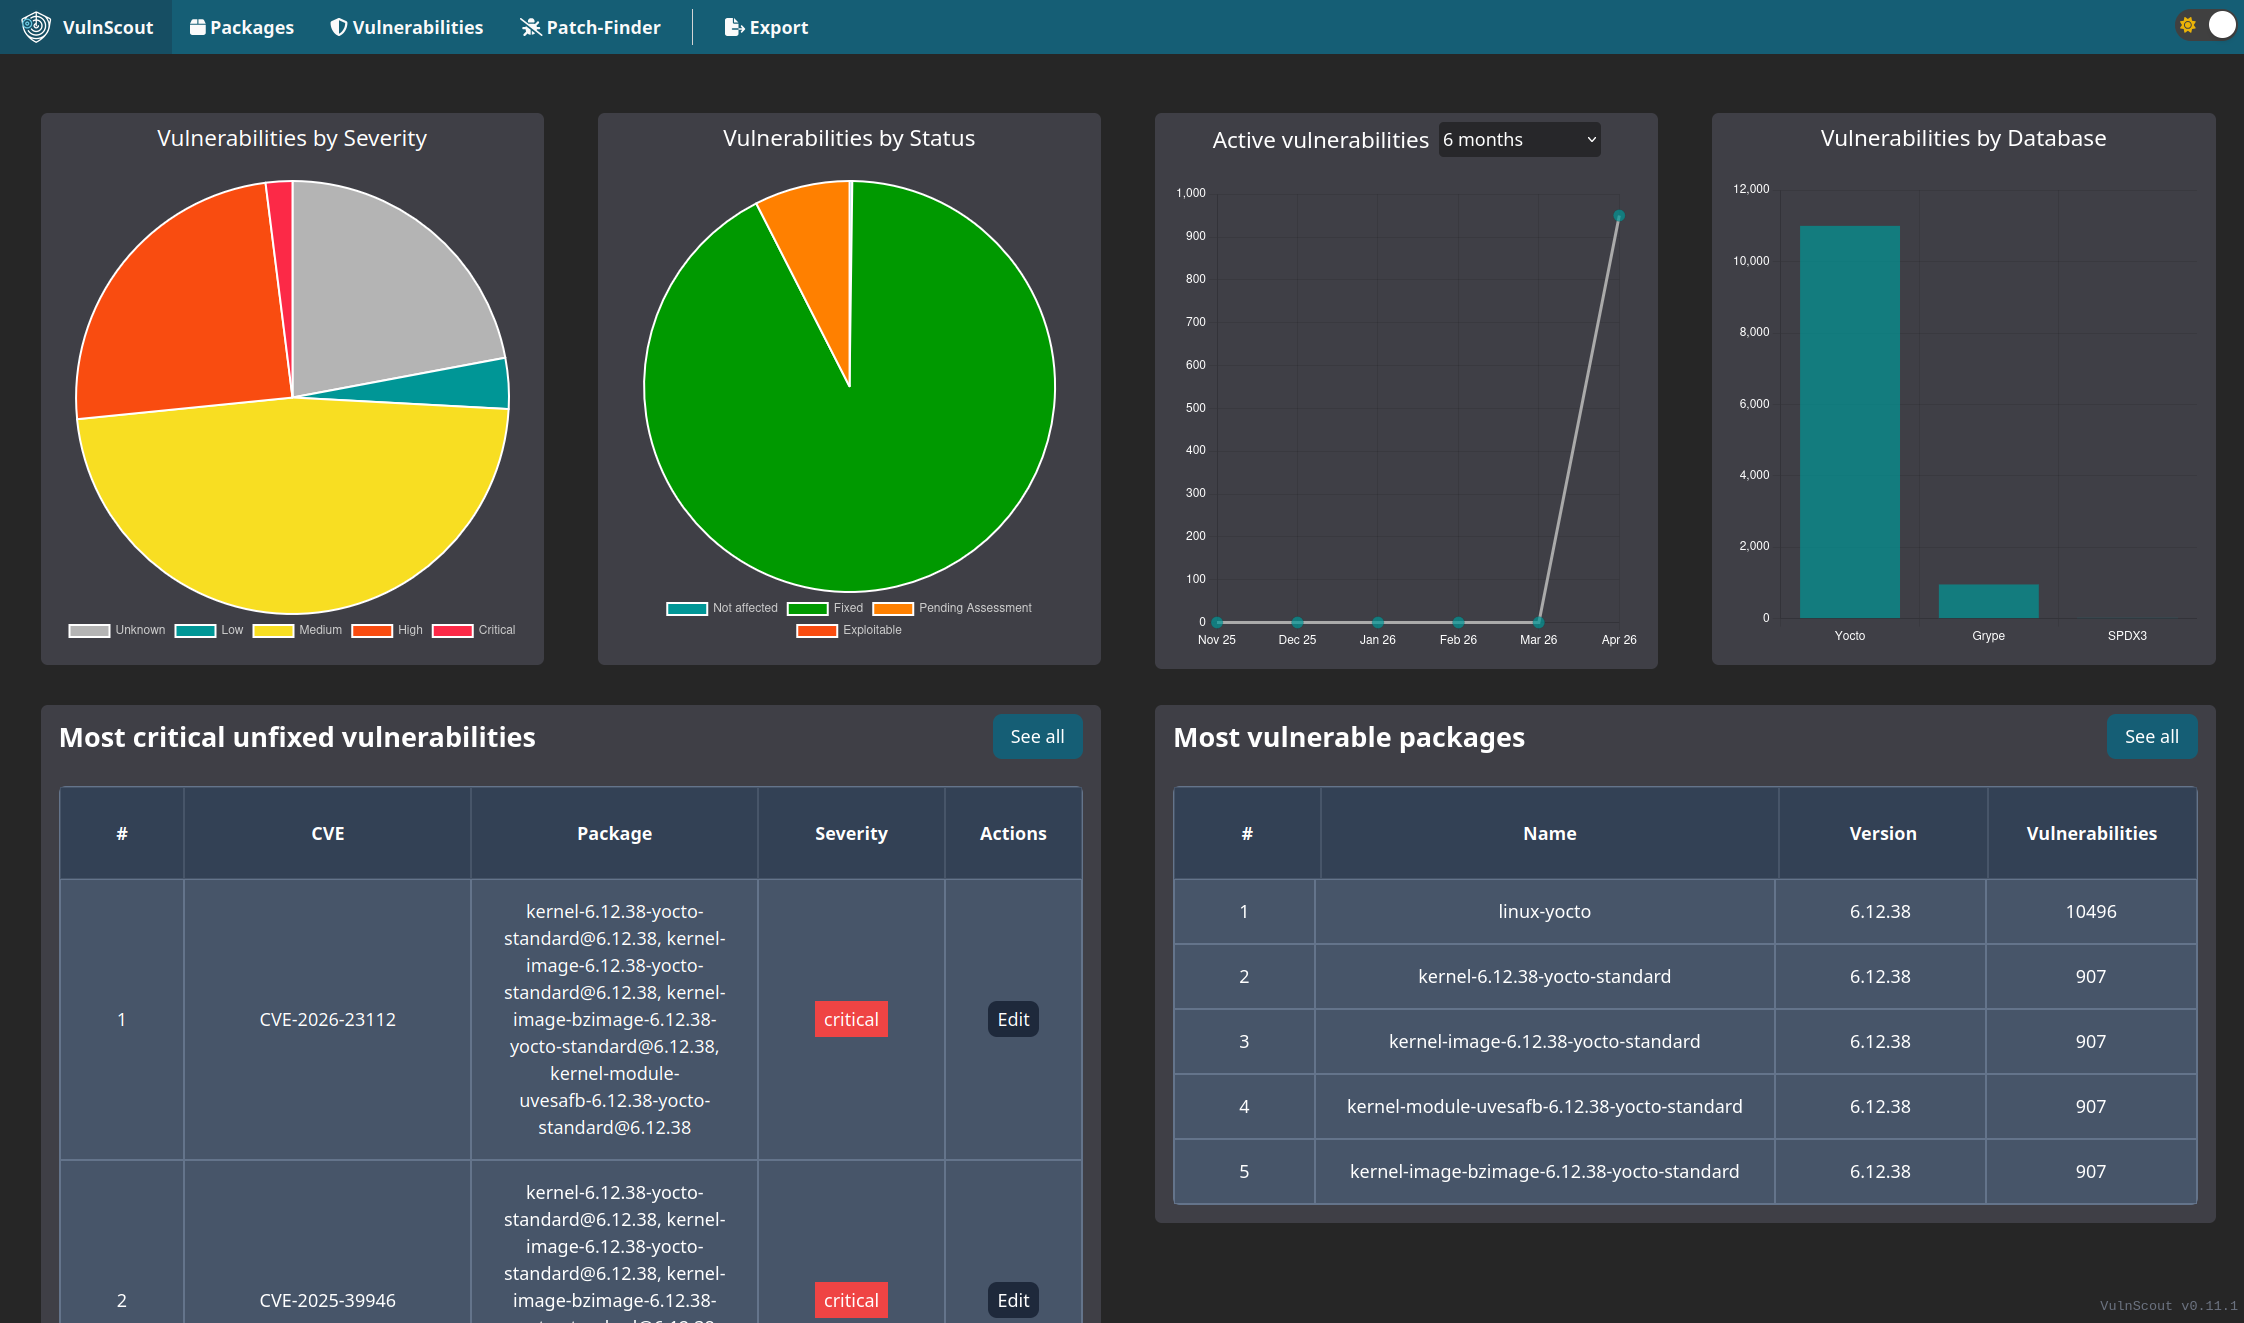
\includegraphics[height=0.8\textheight]{slides/security-compliance/vulnscout.png}
\end{frame}

\begin{frame}{sbom-cve-check}
  \begin{itemize}
    \item Open Source tool from Bootlin
    \item \href{https://github.com/bootlin/sbom-cve-check}{code} - 
          \href{https://sbom-cve-check.readthedocs.io/en/latest/}{documentation}
    \item Written in python, with as few dependencies as possible
    \item SBoM enrichment based on CVE databases: NVD, CVElistV5
    \item Supports SPDX 2.2 (Yocto's format) and SPDX 3
    \item Can take CVE annotations in format:
    \begin{itemize}
      \item simple-annotations (YAML)
      \item Yocto VEX manifest
      \item OpenVEX
    \end{itemize}
  \end{itemize}
\end{frame}

\subsection{Upgrading strategy}

\begin{frame}{Upgrades}
  \begin{itemize}
    \item Updates can be necessary for multiple reasons:
    \begin{itemize}
      \item Patching a security vulnerability
      \item Rotating cryptographic material (e.g. later stage secure boot keys)
      \item Legal obligation (e.g. CRA)
      \item Adding functionality
    \end{itemize}
    \item Some upgrades are simple, e.g. deploying a patch
    \item Version upgrades can be hard, especially when skipping over versions
  \end{itemize}
\end{frame}

\begin{frame}{Picking a version}
  \begin{itemize}
    \item Embedded systems rely on a plethora of Open Source projects
    \item A lot of work is done \textbf{upstream}
    \item When a vulnerability is found or reported, or an important bug is fixed,
	  only \textbf{supported versions} will get the fix
    \item The further one's version strays from a supported version, the harder
          \textbf{tracking} and \textbf{porting} fixes becomes
    \item In terms of security, being on the newest stable version is usually best
    \item The issue is compatibility
  \end{itemize}
\end{frame}

\begin{frame}{Long-Term Support}
  \begin{itemize}
    \item Long-Term Support (LTS) versions stay supported for longer
    \begin{itemize}
      \item Linux kernel LTS versions are supported for 2 years minimum
      \item Yocto LTS versions receive 4 years of support
      \item Buildroot LTSs are supported for 3 \textbf{years} instead of 3 \textbf{months}
    \end{itemize}
    \item This is advertised plainly:
    \begin{itemize}
      \item the Linux kernel has a \href{https://www.kernel.org/category/releases.html}{list of LTS versions}
      \item so does the \href{https://www.yoctoproject.org/development/releases/}{Yocto project}
      \item the same for \href{https://buildroot.org/lts.html}{buildroot}
    \end{itemize}
    \item The \href{https://cip-project.org/}{Civil Infrastructure Platform}
	  aims to extend LTS windows to over 5 years
    \begin{itemize}
      \item consortium of large industry members
      \item under the Linux Foundation
      \item some features are introduced, not just fixes
    \end{itemize}
  \end{itemize}
\end{frame}
